\section{Discussion}
\subsection{Poiseuille Flow}
\subsubsection{Test of the Basic Algorithm}

The constant error of the FD2 method can be explained by the lack of complexity of the test case.
As the theoretical solution, given by Eq. \ref{vali:pflow_navstok} is a polynom of second order,
no higher order terms will occur in the numerical solution.
Hence, the FD2 method is capable of a perfect approximation, independent of the
grid resolution. The remaining error terms, wich are of the order $10^{-8}$
occur due to the round-off error of the single precision floating-point format.

The convergence of the fourth order scheme, which is above second order
reveals that an error exists in the basic implementation of the No-Slip boundaries.
An explanation can be given with a comparison to the theoretical solution.
The second derivative of Eq. \ref{vali:pflow_navstok}  is given by

\begin{align}
    \pdn[^2 v_x]{x^2} = \frac{1}{\Rey}\pdn[p]{x} := C_f\in\mathbb{R}
\end{align}

where $C_f$ is the constant curvature of the theoretical solution in the fluid domain.
The basic algorithm uses a mirroring method at the boundaries of the fluid domain to fulfill the No-Slip condition (see Sec. \ref{sec:cuda_boundaries}).
Let $C_b$ be the curvature of the velocity profile in the boundaries, it follows that $C_b = - C_f$, as a result of the mirroring method.
Therefore a discontinuity of the second derivative is created at the boundaries.
When using FD2 method the 3-Point stencil evaluates to the correct value.
The 5-Point stencil of the FD4 method evaluates to a false value, since it uses one point behind the boundary.
As a result the discontinuity creates an error in this approximation.


\subsubsection{Test of the Volume Penalization Method}

The offset on the boundaries arises since the VP method cannot fulfill the exact boundary conditions.
For the steady state a force equilibrium at the boundaries is given by the pressure gradient, the viscous force and the damping force

\begin{align}
\label{valid:steady_state_pflow}
 \frac{H}{J} v_x &=  \frac{1}{\Rey}\frac{\partial^2 v_x}{\partial z^2} -\pdn[p]{x}.
\end{align}

The result is a constant offset $v_x(h_1) = v_x(h_2) =: C\in\mathbb{R}$.
The simultaneous decrease of the $l_2$-error with $J$ is as expected, since a stronger damping force $\propto \nicefrac{1}{J}$ creates a smaller
error at the boundaries.
However, it is counterintuitive that the $l_2$-error decreases with an increase of the Reynolds number.
An explanation is that the viscous force and the pressure gradient are proportional to $\nicefrac{1}{\Rey}$
(see Eq. \ref{vali:pflow_pcondi}).
With an increase of the Reynolds number the left side of Eq. \ref{valid:steady_state_pflow} becomes smaller,
the damping force becomes larger in comparison and the  offset $C=v_x(h_1)=v_x(h_2)$ decreases.

\begin{figure}[!bp]%
    \centering
    \subfloat[Velocity profile at the immersed boundary for the VP-FD2 and the VP-FD4 method]{{
    \label{fig:example_a}%
      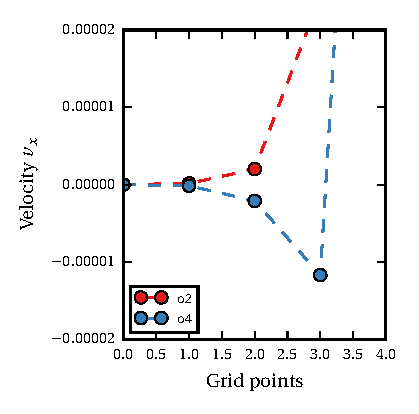
\includegraphics{gfx/immersed_boundary/poiseuille_flow/discussion/stencil.pdf}
            }}%
    \qquad
    \subfloat[Schematic velocity profiles for different resolutions.]{{
    \label{fig:example_b}%
      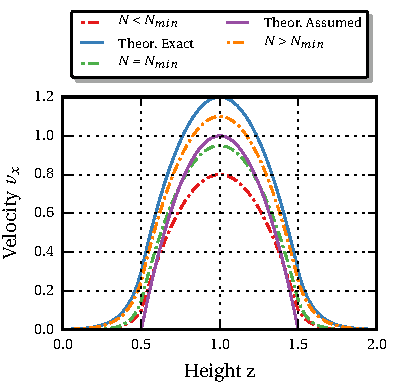
\includegraphics{gfx/immersed_boundary/poiseuille_flow/discussion/profile.pdf}
        }}%
    \caption{}
\end{figure}

The grid convergence study with a constant Reynolds number and variable damping coefficient, generates an error
which increases simultaneously with the grid resolution.
An explanation can by given by revising the theoretical solution
and the finite difference stencils at the fluid boundaries.

The error for both methods does not converge towards zero. This means there has to be some discrepancy to the theoretical solution given by
Eq. \ref{vali:pflow_theosol}.
For a constant $J$ there is an offset $C$ to the theoretical solution,
which is given by the equilibrium accord to Eq.  \ref{valid:steady_state_pflow}.
This further means that the theoretical solution which was assumed in the first place, is wrong for the VP method.
An additional offset in the flow which is dependent on the damping coefficient $J$ has to be considered.
For a low resolution, the profile of the FD2  method is closer to the assumed theoretical one, which results in a smaller
error. With an increase to a higher resolution the error with respect to the real solution decreases.

An explanation for the convergence of the FD4 method can be given by further considering the discretization error at the fluid boundaries.
Fig. \ref{fig:example_a} shows exemplarily the velocity profile near to the fluid boundary, for the Volume-Penalization method of FD2 and FD4 order
at a resolution of $N=100$.
It can be seen that the velocity profile for the FD4  method  is slightly negative.
The reason for this is the use of a 5-Point stencil for the discretization.
The stencil reaches over the immersed boundary which results in a wrong computation of the Laplacian

The  error convergence is a result from  the velocity profiles for different resolutions,
as shown schematically in Fig. \ref{fig:example_b}.
\footnote{The difference in the computed velocity profiles is barely visible. Therefore, an exaggerated version is used.}
The velocity profiles for three different resolutions are considered for a constant $J$,
the minimum of the error shall be defined as $N_{min}$.
Due to the negative velocity at the boundary the first profile $N<N_{min}$ lies below the theoretical solution,
given by Eq. \ref{vali:pflow_theosol}.
The second profile is at $N=N_{min}$. The error at the boundary is smaller due to the increase of the resolution.
The velocity profile overlaps best with the theoretical solution resulting in a minimal error.
With a further increase of the resolution  $N>N_{min}$ the velocity profile drifts away from the theoretical solution.
The error increases.  Finally, the method converges towards the same solution as the second order scheme.


\subsubsection{Test of the Direct Forcing Method}

The constant error of the FD2 can again be explained by the lack of complexity of the test case.
The FD2 method is capable of a perfect approximation and
the remaining error terms of the order $10^{-8}$
occur due to the round-off error of the single precision floating-point format.

In comparison to the basic algorithm which was above second order, the convergence of the FD4 method is above first order.
Once more this error is a result of the used 5-Point stencil.  All values behind the fluid boundary are set
to zero. The 5-Point stencil uses one grid point behind the boundary which results in a incorrect computation.

\subsection{Hagen-Poiseuille Flow}

\label{sec:hpflow_discussion}


The simulation of the Hagen-Poisseuille flow points out multiple numerical problems of the
implementations.
The first which shall be considered is the error in the IP method.
In comparison to the  IP-FD2 method, the IP-FD4 method contains an error which is about one to two orders larger.
Fig.\ref{valid:hpflow_velodiff_discussion} shows the subtracted velocity profiles for the IP-FD4 and FD2 method in the $(y, z)$-plane.
It can be noted that the velocity differences inside of the fluid domain are small but large in the wall region.
Especially close to the fluid boundary the difference  is of order $10^{-2}$.
One explanation for this result is the use of a different stencil for the FD4 scheme.
The 5-Point stencil reaches over the domain boundaries an incorporates errors by a false approximation, similar to the Poiseuille flow.
This is not a problem for the FD2 method due to the use of a 3-Point stencil.
The motivation of the combination of IP and DF methods was to set the velocities in the wall region to zero.
However, the computation is numerically unstable.
\begin{figure}[!tp]
  \begin{minipage}[c]{0.4\textwidth}
      \centering
      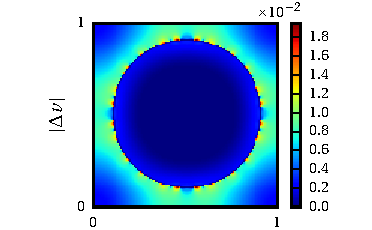
\includegraphics{gfx/immersed_boundary/hpflow/discussion/vzdiff.pdf}
  \end{minipage}
  \begin{minipage}[c]{0.6\textwidth}
      \caption{Absolute value of the velocity difference between the IP-FD2 and IP-FD4 in the (y, z)-plane.
      \label{valid:hpflow_velodiff_discussion}
      }
  \end{minipage}
\end{figure}
One assumption is that this instability is created by the density which is interpolated over the domain boundaries.
The only case in which the wall and the fluid domain are decoupled are the FD2 methods.
Therefore no difference between the IP-FD2 and the IP+DF-FD2 method can be observed.
An additional attempt was made to interpolate the density at the border according to \citep{Gilmanov2003}.
The results are not presented in this thesis, since it turns out that the computation is numerically unstable.

The second problem concerning this numerical implementation, are density oscillations
which occur for the FD4 methods.
One possible explanation for this behaviour might be the odd-even decoupling of the density.
The numercial change in the density is  proportional to \footnote{o.t. = other terms}


\begin{align}
    \frac{\rho^{j+1}_{i} -  \rho^{j}_i}{\Delta t}  \propto \frac{ v^j_{i+1} - v^j_{i-1}}{\Delta x} + \text{o.t.}
     \propto \frac{\rho^{j-1}_{i+2} - 2 \rho^{j-1}_{i}  + \rho^{j-1}_{i-2}}{\Delta x^2} + \text{o. t.}
\end{align}

where $j$ is the time step and $i$ a grid point. Here the one-dimensional case is considered with an FD2 discretization and an explicit Euler step in time.
This means that the density field is implicitly coupled over the velocity to itself,
but neighbor points are independent of each other.\footnote{This example also holds for the FD4 method.}
For the three dimensional setup six decoupled pressure fields would be possible.
From the artificial continuity equation (see Sec. \ref{num:sec_articomp})
it is known that $\partial_t \rho  = \nabla \vec{v} =  0$, which is true for the FD2 case.
The oscillation could be a result of the  wrong computation due to the use of a 5-Point stencil at the boundaries.
Due to the decoupling the computed error evolves differently on the decoupled pressure fields.
%One one pressure field i.e. more errors are computed due to the overlap with the boundarie
%than for another field.
%for the points where the 5-Point stencil reaches over the domain bounday.
%Due to the odd-even decoupling the computed error is different in the grids .
%Overall the oscillation are small and therefore not yet a concern

Finally a comparison of the error shall be given.
In \citep{Fadlun2000} the DF method was tested with and without the VF method.
Furthermore a linear interpolation method, similar to the IP method was used.
As a test case the formation of a vortex ring behind a curvilinear noozle was tested.
The results show that for the DF method the error converges below first order, but can be
improved with the VF method to about first order convergence.
The interpolation method is about second order accurate.
For all methods the error is of order $10^{-2}$ at $N=100$.
This result for the IP-method is in argreement with this thesis. However, the DF-method has a better convergence rate of first order and
the additional use of the VF method has a smaller influence.

A validation of the IP method can be found in \citep{Gilmanov2003}, \citep{Gilmanov2005}.
In \citep{Gilmanov2003} the IP method is tested by the steady flow in a lid-driven cavity containing a sphere, the error convergence of order $1.74$.
In  \citep{Gilmanov2005} a flow caused by an oscillating sphere in a cavitiy is studied, with an error convergence of order $1.77$.
In this thesis the IP-FD2 method has a convergence rate about $2.35$, above second order, which is slightly better in comparison to these validations.
One reason for this could be the lack of complexity in the Hagen-Poiseuille flow as the theoretical solution is a polynom of second order.


\subsection{Taylor-Couette Flow}

In this validation test case the density changes for the FD2 methods as well.
The convergence of the averaged density to the order of $10^{-4}$
is similar to the Hagen-Poiseuille flow with exception of the IP+DF FD2 and DF-VF FD4 method ($\approx10^{-3}$).
The change in density is related to the numerical setup which is more complex in this testcase.
Due to the boundary conditions the divergence of the velocity field is not zero at the start of a simulation.
A density field emerges and grows until a steady state is reached.
This is a result of the method of articficial compressibilty, see Sec. \ref{num:sec_articomp}
Even with the use of a large speed of sound (here $\Mach=\nicefrac{v}{c}\approx0.05$)
the fluid is still not completely incompressible. However, the overall change in density is small.
The spatial oscillations in this test case also occur in the FD2 methods since the density is no longer zero.
It can be assumed that just like in the Hagen-Poiseuille flow an odd-even decoupling occurs.
The decrease of the density in the inner cylinder for the VP-method can assumed to be physically correct.
The angular velocity $\Omega_i$ creates a centrifugal force in the inner cylinder,
This results in a density distribution which is large at the outer cylinder walls and small in the center.
The negative value is not a concern since the density is undetermined by a constant.

It can be noted that the results of the IP FD2 and the IP+DF FD2 method are not equal.
This refutes the previous assumption (see Sec. \ref{sec:hpflow_discussion}),
that the velocity fields of the fluid domain and the boundaries are decoupled for FD2 methods.

For the DF and VP methods the error and convergence rates are similar,
but the error of the IP methods is about one order higher in comparison to the Hagen-Poiseuille flow.
The use of the VF method leads to an increase of the overall error, which is contrary to results of the Hagen-Poiseuille flow.

The velocity difference profiles for all methods (Fig. \ref{tcflow:results_vprofiles_o2} and Fig. \ref{tcflow:results_vprofiles_o4})
indicate a erroneous approximation of the inner boundary.
Hence, it can be assumed that the approximation of Dirichlet boundaries, with velocities differing from zero at the boundaries,
creates an overall larger numerical error.

A comparison to results in litetature is difficult.
THere

%- nicht auszuschliefen wegen druckmethode blabla
%-a comparison to literature ...
%- studies with moving boundaries where blab la howvere this cannot be compared

%-short comp literature?
%-not found bot oscillation with moving boundaries
%However, it is noticeable that for the DF methods the density in the inner cylinder is zero, see Appendix \ref{tcflow:results_rho_profiles_o2}.
%Since the velocities are directly set to $\vec{\Omega_i} \times \vec{r}$ in the inner cylinder,
%the fluid can be considered incompressible in this domain because $\partial_t \rho = \nabla (\vec{\Omega_i} \times \vec{r}) = 0$.
%
%Fig.\ref{valid:hpflow_velodiff_discussion} shows the subtracted velocity profiles for the IP FD2 and IP+DF FD2 method in the $(x, y)$-plane.
%The largest differences between these profiles occur at the boundary of the inner cylinder, about $10^{-2}$.
%Both methods create different numerical approximations at this location.
%
%\begin{figure}[!bp]
%  \begin{minipage}[c]{0.4\textwidth}
%      \centering
%      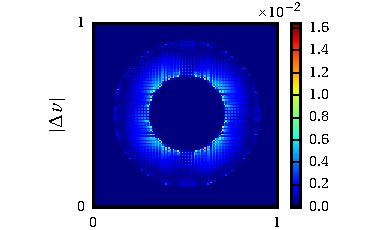
\includegraphics{gfx/immersed_boundary/tcflow/discussion/vzdiff.pdf}
%  \end{minipage}
%  \begin{minipage}[c]{0.6\textwidth}
%      \caption{Absolute value of the velocity difference between the IP-FD2 and IP+DF-FD2 in the (x, y)-plane.
%      \label{valid:hpflow_velodiff_discussion}
%      }
%  \end{minipage}
%\end{figure}

%This is not unexpected for the VP and DF methods, since a pixelated moving boundary probably creates a to the roughness of the surface.
%From the velocity profiles it can be seen that the error of the interpolation methods is smaller at the inner boundaries.
%But still the error here is larger at the outer boundaries which indicates that moving boundaries are also difficult to interpolate with good results.

\clearpage

\section{Summary}

In the first part of the chapter an introduction to different Immersed Boundary methods was given.
The volume-penalization method, adapted from  \citep{Lulff2011} uses a forcing term which is proportional to the velocities at the fluid boundaries.
In case of the Direct-Forcing method, adapted from \citep{Fadlun2000} the forcing term is calculated implicitly.
Both methods were extended by the Volume-Fraction method, adapted from \citep{Fadlun2000}, which computes the fluid domain volume ratio inside a boundary
cell and uses this value as a weighting coefficient for the forcing.
Finally an interpolation method adapted from  \citep{ Gilmanov2003} was introduced. In the first step this method performs a bilinear interpolation on a surface
next to the fluid boundary, in the second step this value is linear interpolated to a grid point close to the boundary.

In the second part of the chapter three different test cases were introduced as a validation for the Immersed Boundary methods.
The laminar Poiseuille flow was used as a first validation test case for the DF and VP methods.
From the results it was possible to identify an error in the basic algorithm of the simulation.
Furthermore it could be shown that the use of a 5-Point stencil leads to discretization errors at the fluid boundaries.

In the second test case a simulation of a Hagen-Poiseuille flow was performed.
The results of this simulation pointed out possible numerical issues.
One possible problem are numerical oscillations which are assumed to be caused
by a decoupling of density field.
Furthermore this test case showed that the use of a 5-Point stencil creates a numerical error,
which results in a large error for the IP-DF4 method.
It can be noted that using the volume fraction method  the error of the DF and VP method can be improved.
In summary all errors are approximately below the order  $10^2$ for $N>100$,
by far the smallest error was obtained with the IP-DF2 method.
All convergence rates are at least as good in a comparison
to the results from validation test cases from literature.

The last test case was given by a Taylor-Couette system.
In comparison to the Hagen-Poiseuille flow the computed numerical error is larger,
up to an order for the VF methods, which perform inferior in this test case.
In this simulation for both the FD2 and FD4 methods small pressure oscillations can be observed which are again assumed to be
caused by a decoupling of the density field.
The velocity profiles show that the error is the largest to the inner domain boundary $r_i$.
This indicates that the Immersed Boundary methods in combination with implemented basic GPU algorithm
are not a good choice for moving boundaries.





